\chapter{Formulação do Problema}\label{chapter:formulacaoDoProblema}

O desenvolvimento da plataforma \textit{Corporate Collaboration} pretende atingir certos requisitos, de forma a poder enquadrá-la no mercado 
atual. 


\section{Estado da Arte}\label{sec:estadoDaArte}
As plataformas de colaboração existentes no mercado atual tais como a \textit{Microsoft SharePoint} ou a \textit{BaseCamp} apresentam um elevado nível de complexidade, 
incluindo ferramentas como calendários partilhados, partilha de ficheiros, mensagens instantâneas, armazenamento na \textit{cloud}, video-conferência, entre outros. 
A aplicação desenvolvida neste âmbito não procura igualar todas as funcionalidades das plataformas já existentes, 
mas sim, agilizar a dinâmica de atividades internas que ocorrem diariamente nas empresas. 
Visa, essencialmente, facilitar a procura de pessoas para cumprir certas necessidades que existam no âmbito das atividades internas da empresa, 
necessidades estas que permitem definir uma tarefa que tem de ser realizada ou um evento que será organizado no contexto da dinâmica interna da empresa. 
Estas necessidades são auxiliadas por recursos que permitem gerir candidaturas e participantes das mesmas, 
assim como apresentar informações sobre alojamento, refeições, transporte e localização, se for caso disso.

\section{Análise de Requisitos}\label{sec:requisitos}

As funcionalidades principais da plataforma \textit{Corporate Collaboration} estão representadas na figura~\ref{fig:uc:generalActions}

\begin{figure}[H]
    \centering
    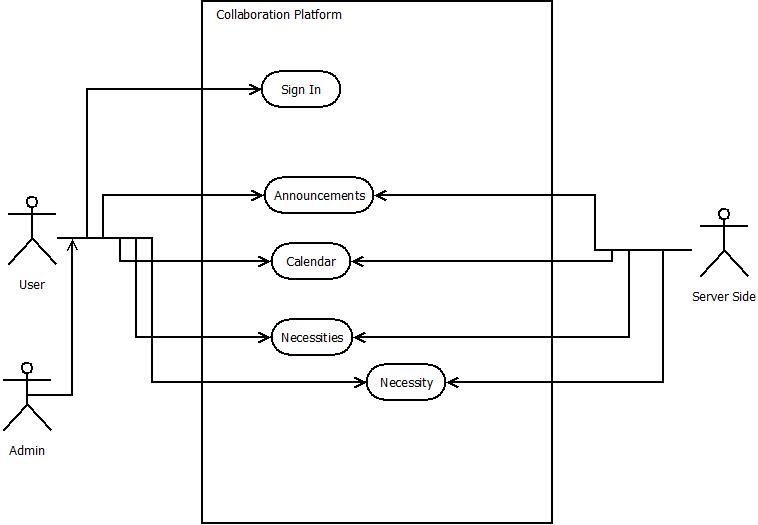
\includegraphics[scale=0.6]{figures/General Actions.jpeg}
    \caption{\textit{Use Case} --- Ações gerais.}\label{fig:uc:generalActions}
\end{figure}

\subsection{Registo e Autenticação}\label{subsec:login}
Para desenvolver a funcionalidade de registo e autenticação na plataforma de colaboração é necessário existir uma tabela 
na base de dados que guarde as credenciais e informação básica de cada utilizador, nomeadamente 
o \textit{email}, \textit{password}, \textit{username}, primeiro e último nome. 
Esta tabela tanto serve para efeitos de registo de um utilizador, como para verificação posterior da sua autenticação. 
Os utilizadores não necessitam de fazer registo na aplicação, visto que nesta plataforma é suposto utilizarem 
as mesmas credenciais atribuidas pela empresa, para e-mail e autenticação nas outras aplicações internas.

Relativamente ao ecrã de \textit{Login} ilustrado na figura~\ref{fig:uc:login}, este suporta:

\begin{itemize}
    \item Duas caixas de texto onde o utilizador introduz o seu e-mail e password.
    \item Um botão identificado como \textit{Login} que desencadeia o processo de verificação das credencias introduzidas.
\end{itemize}

\begin{figure}[H]
    \centering
    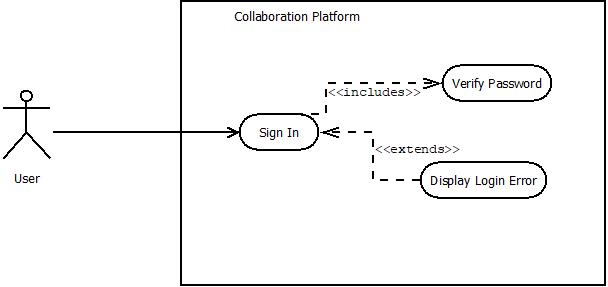
\includegraphics[scale=0.6]{figures/Login Use Case.jpeg}
    \caption{\textit{Use Case} --- \textit{Login}.}\label{fig:uc:login}
\end{figure}

O utilizador com permissões de administrador tem acesso ao \textit{back-office} onde pode criar ou remover categorias.

\subsection{\textit{Home Page --- Dashboard}}\label{subsec:dashboard}

Após o \textit{login} na aplicação o utilizador será redirecionado para um novo ecrã que irá conter um \textit{dashboard} com o intuito de organizar e 
apresentar a informação de uma forma apelativa. As necessidades a que o utilizador se candidatou serão apresentadas neste \textit{dashboard}. 
O mesmo irá conter também uma secção com estatística relativa ao número de necessidades que existem em cada categoria. 
A seleção de uma das categorias na estatística redirecionará o utilizador para o ecrã das necessidades, 
apresentando a lista das mesmas com o filtro correspondente à categoria selecionada. 

\subsection{Registo das necessidades internas da empresa, gestão de candidaturas, notificações e integração com o google maps}\label{subsec:necessitiesCandidatesNotificationsGoogleMaps}

A funcionalidade de registo de necessidades internas da empresa estão organizadas em categorias de modo a facilitar a navegação do utilizador pelas mesmas.

\begin{figure}[H]
    \centering
    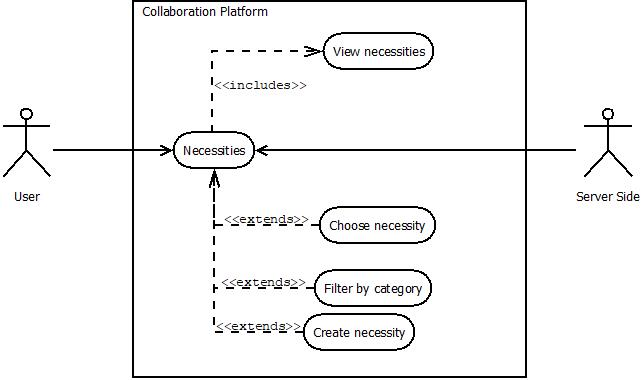
\includegraphics[scale=0.6]{figures/Necessities.jpeg}
    \caption{\textit{Use Case} --- Necessidades.}\label{fig:uc:necessities}
\end{figure}

Para isso, é fundamental que exista um ecrã que apresente todas as necessidades da empresa. 
Um utilizador, caso queira registar uma necessidade, irá escolher a categoria que melhor se adequa à mesma. 
Caso não exista, este, se tiver permissões de admin, poderá criar uma categoria nova no \textit{back-office} da aplicação. 
Neste ecrã será possível filtrar as necessidades pela sua categoria e pelo seu grau de urgência.

\begin{figure}[H]
    \centering
    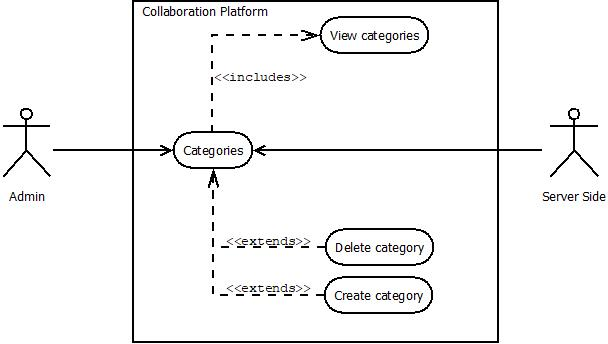
\includegraphics[scale=0.6]{figures/Categories use case.jpeg}
    \caption{\textit{Use Case} --- Categorias.}\label{fig:uc:categories}
\end{figure}

Posto isto, definimos um conjunto de filtros que podem ser conjugados de modo a permitir um melhor agrupamento e organização das necessidades. O primeiro consiste na filtragem por categorias, como por exemplo \textit{Brown Bags}, 
\textit{Qualification Offers}, \textit{Software Components Development} ou \textit{Planning of Events}. 
Foi ainda definido um segundo filtro que poderá tomar os valores \textit{High}, \textit{Medium} ou \textit{Low}, 
correspondentes ao grau de prioridade com que as necessidades foram criadas. 
A seleção dos filtros irá levar a uma atualização da lista para conter apenas necessidades que se enquadrem nessa mesma seleção. 
Este ecrã apresenta ainda um botão que servirá para criar uma nova necessidade, criação esta acessível a todos os utilizadores autenticados, 
que decorrerá num novo ecrã e que terá como opção (obrigatória) de criação os filtros a qual associar a nova necessidade. 
Em cada necessidade existe a possibilidade de associar recursos com informações sobre alojamento, refeições, localização do evento ou transporte para o local onde a mesma se irá realizar. Todos os recursos, com exceção do recurso transporte, têm associado um mapa do \textit{Google Maps} onde os utilizadores podem fornecer informações sobre localização.
Ao clicar numa necessidade, será apresentado um novo ecrã com os detalhes da mesma, com os recursos associados e também a possibilidade do utilizador se candidatar como colaborador ou participante da necessidade, dependendo da fase em que a mesma se encontra. O autor da necessidade irá receber a notificação de que existe um novo candidato, 
dando-lhe a opção de após carregar na notificação ser redirecionado para o ecrã de detalhe da necessidade onde pode observar os candidatos. 
Ao criar uma necessidade o autor tem a possibilidade de escolher se todas as candidaturas à necessidade em causa são aceites automaticamente ou se o próprio escolhe os candidatos com base na descrição dada pelos mesmos.  
O candidato irá receber uma notificação nos casos em que a necessidade for fechada/cancelada, e quando a sua candidatura for aceite/recusada. 
Terá também a possibilidade de ver quem já se candidatou á necessidade criada pelo próprio no ecrã de detalhe na parte dos participantes, estando candidatos a colaboradores separados de candidatos a participantes. 
O ecrã que permite mostrar as notificações associadas a cada utilizador é acedido ao carregar no ícone em forma de sino presente na barra da aplicação. Este ícone tem um pequeno contador associado que indica o número de notificações pendentes que cada utilizador tem e, quando pressionado, é apresentado o ecrã das notificações onde as mesmas são apresentadas na forma de uma lista. 

\begin{figure}[H]
    \centering
    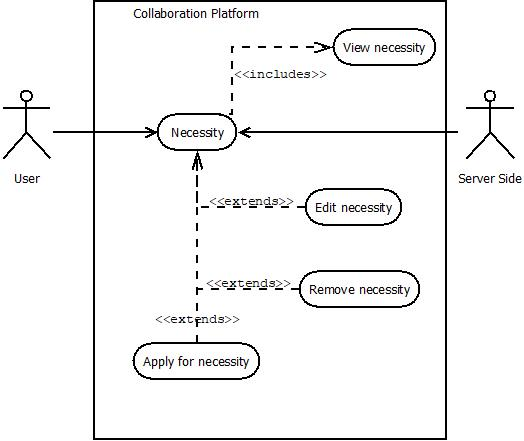
\includegraphics[scale=0.6]{figures/Necessity.jpeg}
    \caption{\textit{Use Case} --- Necessidade.}\label{fig:uc:necessity}
\end{figure}

Exemplificando, para organizar eventos ou feiras de emprego, o utilizador seleciona a categoria \textit{Planning of events}.

Se por outro lado, tivermos o objetivo de realizar apresentações informais de partilha de conhecimento o utilizador seleciona a categoria \textit{Brown Bags}. 
Todos os utilizadores devidamente autenticados podem candidatar-se para assistir a uma dada apresentação ou para a orientar. 
No contexto da necessidade é definida uma linha temporal que consiste numa primeira fase de candidaturas para escolha do orientador 
(ou orientadores) que irão conduzir a apresentação, seguida de uma segunda fase de candidaturas para utilizadores que queiram assistir à apresentação. 
O autor de uma apresentação, no ecrã de detalhe da mesma, terá acesso a quem se candidatou para a orientar, podendo escolher um ou mais orientadores 
com base na descrição apresentada pelos mesmos. 
Numa segunda fase após a escolha do(s) mesmo(s), o autor pode ver os utilizadores que se 
candidataram à necessidade no seu ecrã de detalhe e todos os utilizadores autenticados podem ver quem foi aceite/vai ao evento.

%%%%%%%%%%%%%%%%%%%%%%%%%%%%%%%%%%%%%%%%%%%%%%%%%%%%%%%%%%%%%%%%%%%%%%%%%%%%%%%%%%%%%%%%%%%%%%%%%%%%%%%%%%
\comment{
    A categoria \textit{Make a Post} tem como objetivo a criação de um post numa rede social ou blog. 
    O utilizador ao filtrar esta categoria ser-lhe-á apresentado a lista dos posts. 
    O utilizador ao carregar num post navegará para um novo ecrã que apresentará os detalhes do mesmo. 
    Os detalhes apresentados para um post já publicado incluem uma breve descrição, um link para o post e a pessoa que o realizou. 
    Os detalhes para um post não publicado incluem a possibilidade de o utilizador se candidatar para o realizar, assim como uma breve descrição.

    Com o objetivo de possibilitar ofertas de formação dentro da empresa, foi definida a categoria \textit{Qualification Offers}. 
    Esta categoria apresenta uma dinâmica semelhante à categoria \textit{Informal Presentations}, visto que ambas procuram a partilha de 
    conhecimento por parte de um ou mais oradores, definidos numa primeira instância, seguida de uma segunda fase em que os utilizadores 
    poderão manifestar a sua intenção em participar. 
    O principal fator que distingue estas duas categorias é a duração da atividade: 
    uma oferta de formação decorrerá ao longo de várias sessões satisfazendo um número total de horas apresentado na descrição da necessidade, 
    ao contrário de uma apresentação informal que é um acontecimento único de duração na ordem dos minutos. 
    Posto isto, a dinâmica apresentada nesta categoria quanto ao ecrã de detalhes e metodologia será semelhante à da categoria \textit{Brown Bags}.

    A categoria \textit{Software Components Development} tem como objetivo propor projetos e procurar participantes para os mesmos, no âmbito de desenvolvimento de software. 
    Ao ser selecionada uma proposta será apresentado um novo ecrã com a sua descrição, detalhes e com um botão que permitirá ao utilizador 
    candidatar-se para integrar o projeto.

    Com o objetivo de proporcionar oportunidades de progressão na carreira de forma espontânea, por exemplo, 
    haver uma vaga para uma posição de tech lead num novo projeto, e os seniors interessados poderem candidatar-se a esta posição. 
    O utilizador após selecionar a categoria \textit{Opportunities for Career Progression} serão apresentadas todas as necessidades correspondentes, sob a forma de uma lista.

    A categoria \textit{Off-work Activities} permite a criação de necessidades com o intuito de realizar atividades lúdicas.
    Um autor desta atividade tem de endereçar os meios de transporte bem como se existe almoço e/ou jantar e as ementas para a respetiva refeição. 
    A funcionalidade de candidaturas nesta categoria funciona de forma a que cada utilizador manifeste a sua vontade em participar no evento.
    Antes do \textit{deadline} desta atividade o utilizador tem de confirmar a sua participação.
}
%%%%%%%%%%%%%%%%%%%%%%%%%%%%%%%%%%%%%%%%%%%%%%%%%%%%%%%%%%%%%%%%%%%%%%%%%%%%%%%%%%%%%%%%%%%%%%%%%%%%%%%%%%
\subsection{Divulgação e calendarização das necessidades}

Com o objetivo de divulgar e calendarizar as necessidades internas da empresa, a barra de navegação da aplicação terá um botão que, quando carregado, 
redireciona o utilizador para um ecrã que apresenta um calendário com o qual ele poderá interagir. 
Neste calendário são apresentados todos os eventos organizados, na sua respetiva data, e existe a possibilidade de filtrar os eventos em que o mesmo participará. 
Após a seleção de um dia no calendário, são apresentados os eventos, dando a possibilidade ao utilizador de ver os detalhes individuais após carregar num deles, 
num novo ecrã.

\begin{figure}[H]
    \centering
    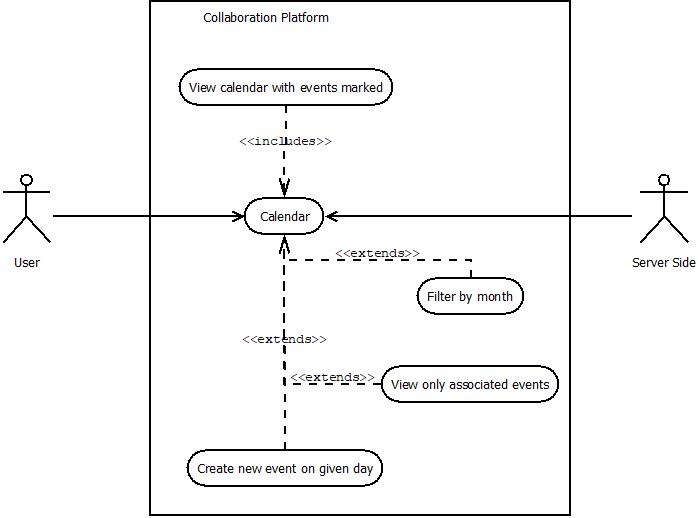
\includegraphics[scale=0.6]{figures/Calendar use case.jpeg}
    \caption{\textit{Use case} --- Calendário.}\label{fig:uc:calendar}
\end{figure}

Para ser possível divulgar as necessidades da empresa de forma uniforme por todos os seus colaboradores, a barra de navegação da aplicação apresentará 
um botão denominado \textit{Announcements} que, quando carregado, abre um ecrã  (figura~\ref{fig:uc:announcements}) que contém os comunicados sobre a forma de uma lista. 
Sempre que for emitido um novo comunicado todos os utililizadores recebem uma notificação com o título do mesmo e, ao carregar nessa notificação, são redirecionados para os detalhes do comunicado. 
Estes comunicados foram criados por um utilizador com permissões de administrador, sendo visíveis por todos os que estejam autenticados.

\begin{figure}[H]
    \centering
    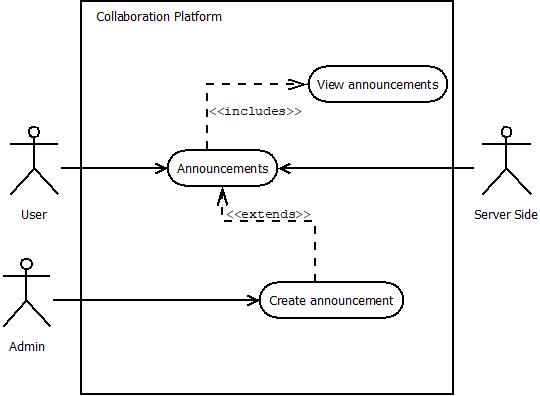
\includegraphics[scale=0.6]{figures/Announcements use case.jpeg}
    \caption{\textit{Use case} --- Announcements.}\label{fig:uc:announcements}
\end{figure}

\section{Plataforma OutSystems}\label{sec:plataformaOutSystems}

A escolha da plataforma \textit{OutSystems~\cite{outsystems}}, para a implementação deste projeto baseia-se essencialmente no facto da mesma ser \textit{low-code},
apresentando vários benefícios essenciais para um projeto de curto prazo como o apresentado. A rapidez
com que é possível produzir peças de \textit{software}, as funcionalidades \textit{user-friendly} como \textit{drag and drop} e 
interfaces de utilizador pré-feitas e a possibilidade de produzir aplicações automaticamente através de
um simples clique, são elementos essenciais que levaram à escolha desta plataforma. 
Cada \textit{endpoint} da aplicação está associado a um ecrã com o qual o utilizador interage, havendo uma navegabilidade entre ecrãs que permitindo, assim,
 que o utilizador visite os diferentes \textit{endpoints} da aplicação.
A criação e utilização de \textit{blocks} é uma das funcionalidades altamente vantajosas que a plataforma \textit{OutSystems~\cite{outsystems}} apresenta, 
visto que permite a reutilização deste componente ao longo da \textit{User Interface --- UI}.
A construção da aplicação torna-se bastante rentável, em termos de tempo e facilidade do desenvolvimento, 
através da conjugação de conceitos como \textit{Widgets}, \textit{Screens} e \textit{Blocks} no domínio da  \textit{UI} 
e de conceitos como \textit{Server Actions} (ações executadas do lado do servidor), \textit{Client Actions} (ações executadas do lado do cliente) 
e \textit{Aggregates} (ação com o propósito de aceder à base de dados para retornar informações persistentes na mesma).
Também é disponibilizado pela \textit{OutSystems~\cite{outsystems}}, um \textit{eSpace} por \textit{module} que contém elementos essenciais 
ao desenvolvimento, como os enunciados anteriormente.
A base de dados está alojada numa \textit{cloud}, onde são guardadas todas as entidades dos vários módulos.
